%!TEX root = main.tex
\section{Experimental Results}
\label{sec:results}

All CGRA cycle counts in Section~\ref{subsec:sbox-comparison}  are obtained from the ESL-CGRA simulator~\cite{Aspros_2025} (deterministic mode).
Section~\ref{subsec:rtl-poseidon2} reports steady-state RTL measurements from Verilator cycle-accurate simulation of the HEEPsilon SoC (ultra-low power CV32E20 host, RV32IMC, single-issue in-order). CPU-only time is derived at \MetricRtlCpuClockMHz\,MHz, whereas CGRA deployments on the OpenEdgeCGRA 4$\times$4, 32-bit datapath use \MetricRtlCgraClockMHz\,MHz. CPU energy follows a fixed CV32E20 reference model of \mw{\MetricRtlCpuPowerModelMW} applied to active-cycle counts; CGRA energy comes from the ESL simulator replay of the deployed kernels. The full Poseidon2 RTL data additionally includes a canonical-state replay with exact agreement to the reference.

\subsection{S-box Kernel Comparison}
\label{subsec:sbox-comparison}

We evaluate three approaches to mapping the S-box kernel
onto the CGRA:
(1)~a hand-optimized schedule (Manual),
(2)~the Compigra compiler~\cite{compigra}, and
(3)~\castm{}, our approach.
Table~\ref{tab:sbox-comparison} summarizes the ESL-measured results; Fig.~\ref{fig:sbox-comparison} presents a visual comparison along with the estimated energy per invocation~\cite{Aspros_2025}.

\begin{table}[t]
\caption{S-box kernel: comparison of compilation approaches under ESL-CGRA simulation.
$NB$: number of compiled bundles; $CC$: clock cycles including stalls;
Disp.: number of CGRA dispatches; Idle (\%): idle-PE ratio, summarized as a bundle-wise geometric mean.}
\label{tab:sbox-comparison}
\centering
\footnotesize
\begin{tabular}{@{}l|rrrr@{}}
\toprule
\textbf{Approach~~} & \boldmath{$NB$} & \boldmath{$CC$} & \textbf{Disp.} & \textbf{Idle (\%)} \\
\midrule
Manual     & \MetricSboxManualNB     & \MetricSboxManualCC     & \MetricSboxManualDispatches   & \pct{\MetricSboxManualIdlePct} \\
Compigra   & \MetricSboxCompigraNB & \MetricSboxCompigraCC & \MetricSboxCompigraDispatches & \pct{\MetricSboxCompigraIdlePct} \\
\castm{}   & \bf{\MetricSboxCastmNB}      & \bf{\MetricSboxCastmCC}     & \MetricSboxCastmDispatches   & \bf{\pct{\MetricSboxCastmIdlePct}} \\
\bottomrule
\end{tabular}
\end{table}

\begin{figure}[hbt]
    \centering
    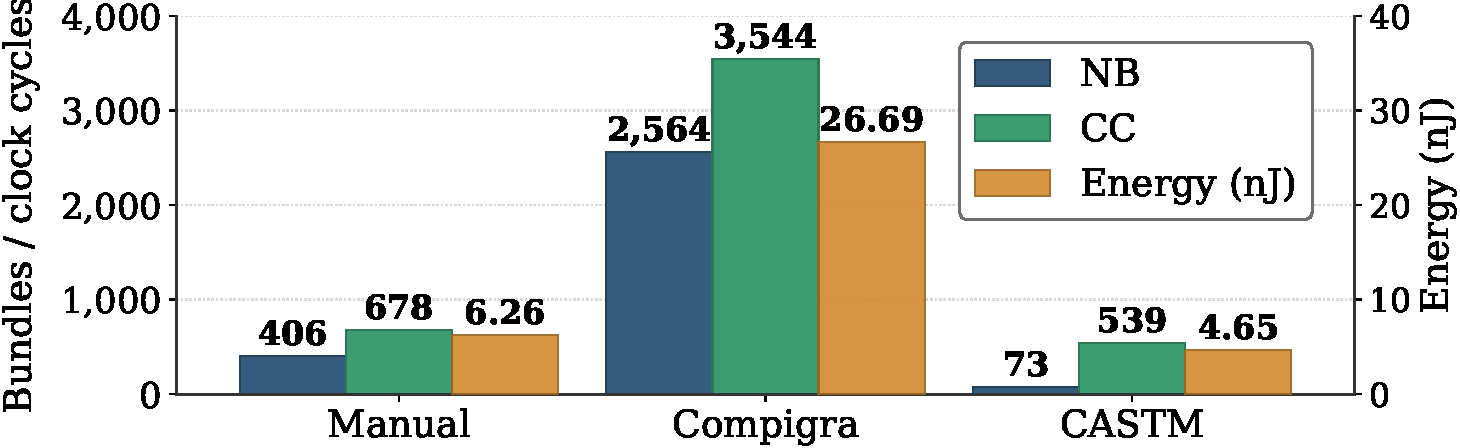
\includegraphics[width=\linewidth]{figures/sbox_compare_plot_v2.pdf}
    \caption{Comparison of the S-box kernel mappings produced by  Manual, Compigra, and \castm{} on the CGRA. Blue and green bars use the left axis and report the number of compiled bundles (NB) and clock cycles (CC), respectively; orange bars use the right axis and report energy (nJoules) per invocation.}
    \label{fig:sbox-comparison}
\end{figure}

Energy per invocation combines the ESL-reported execution energy with the fixed dead-time cost incurred at each CGRA dispatch. This normalization is necessary because the three mappings differ not only in cycle count but also in execution granularity: without accounting for dispatch overhead, a fragmented schedule would understate the system-level cost of repeatedly launching and draining the accelerator.
Idle (\%) in Table~\ref{tab:sbox-comparison} is reported as a bundle-wise geometric mean over per-bundle idle-PE ratios.

\textbf{Compigra cannot map S-box directly.}
The automatic compiler's scheduling heuristic fails on the S-box kernel because Barrett reduction requires cross-PE carry chains and branchless conditional selects that exceed its mapping capabilities.
The workaround is to manually decompose $x^7 \Mod p$ into sub-kernels
and iteratively subdivide when compilation fails---a trial-and-error process that negates the ``automatic'' premise.
The result is \MetricSboxCompigraDispatches{} dispatches with \pct{\MetricSboxCompigraIdlePct} Idle and \pct{\MetricSboxCompigraSmulPct} of SMUL utilization: the hardware multiplier is never used, and the CGRA spends most cycles idle while data is shuffled between dispatches.

\textbf{\castm{} achieves the lowest cycle count.}
The \MetricSboxCastmNB{} compiled bundles (vs.\ \MetricSboxManualNB{} for the Manual schedule) reflect jump-reuse subroutines that share Barrett reduction across the four modular multiplications ($x^2$, $x^3$, $x^4$, $x^7$).
The resulting \cc{\MetricSboxCastmCC} (vs.\ \cc{\MetricSboxManualCC} for Manual) represents a \pct{\MetricSboxCastmCycleReductionPct} cycle reduction attributable to better PE utilization: \pct{\MetricSboxCastmIdlePct} Idle (vs.\ \pct{\MetricSboxManualIdlePct}) and active use of the hardware multiplier (\pct{\MetricSboxCastmSmulPct} SMUL).
Under the energy model, \castm{} also remains the most efficient mapping at \nj{\MetricSboxCastmEnergyNJ}, below Manual at \nj{\MetricSboxManualEnergyNJ} and far below Compigra at \nj{\MetricSboxCompigraEnergyNJ}. The gap is architecturally coherent with the schedules themselves: Compigra expands the kernel into \MetricSboxCompigraDispatches{} dispatches, so its higher energy reflects not only a longer execution (\cc{\MetricSboxCompigraCC}) but also repeated launch and quiescent overheads that are largely avoided by the single-dispatch in the \castm{} schedule.

\textbf{Productivity.}
The Manual approach requires \lines{\MetricLocManual}; \castm{} requires \lines{\MetricLocCastm}---an approximately \timex{\MetricLocCompressionVsManual} reduction.
This gap is structural: \castm{}'s parameterized functions and loop express the kernel once, whereas the hand-written schedule must spell out each PE-cycle placement explicitly, making coding slower and substantially more error-prone.

\textbf{Code complexity.}
Table~\ref{tab:halstead} quantifies complexity using Halstead active volume metric, $V_{\text{act}} = N \log_2 \eta$, where $N$ counts active (non-NOP) tokens~\cite{halstead1977}. We do not report Halstead effort because, for low-vocabulary ISA-level code, it can produce anomalous scaling~\cite{sinha2011}. Owing to explicit per-PE-per-cycle encoding, the Manual schedule reaches \timex{\MetricHalsteadManualRatio} the \texttt{C++} baseline. By absorbing spatial placement and NOP scheduling into the compiler, \castm{} reduces this to \timex{\MetricHalsteadCastmRatio}, corresponding to a \timex{\MetricHalsteadCompressionVsManual} compression factor relative to the Manual schedule. Ideally, Compigra could reduce this complexity to \timex{\MetricHalsteadCompigraRatio} the \texttt{C++} baseline, although at the cost of \timex{\MetricSboxCompigraSlowdownVsCastm} more cycles than \castm{} due to inefficient PE utilization as previously explained.

% AUTO_HALSTEAD_TABLE_BEGIN
\begin{table}[ht]
\caption{Halstead metrics for the S-box kernel. LOC: source lines; $\eta$: unique vocabulary; $N$: active tokens (NOP excl.); $V_{\text{act}}=N\log_2\eta$: active volume~\cite{halstead1977}; Ratio: $V_{\text{act}}$ norm.\ to C++.}
\label{tab:halstead}
\centering
\scriptsize
\setlength{\tabcolsep}{2pt}
\begin{tabular}{@{}l|rrrrr@{}}
\toprule
\textbf{Approach} & \textbf{LOC} & \boldmath{$\eta$} & \boldmath{$N$} & \boldmath{$V_{\text{act}}$} & \textbf{Ratio} \\
\midrule
C++ (Ref.) & 25 & 39 & 104 & 550 & $1.0\times$ \\
Compigra & 47 & 53 & 227 & 1{,}300 & $2.4\times$ \\
Manual CSV & 2{,}030 & 48 & 6{,}348 & 35{,}453 & $64.5\times$ \\
\castm{} (\textbf{Ours}) & \textbf{340} & \textbf{55} & \textbf{607} & \textbf{3{,}509} & $\mathbf{6.4\times}$ \\
\bottomrule
\end{tabular}
\end{table}

% AUTO_HALSTEAD_TABLE_END

\subsection{S-box Configuration Register Pressure}
\label{subsec:creg-analysis}

The S-box kernel also allow us to conduct a controlled sensitivity study for configuration residency. Two implementations bracket the design space: the \emph{Manual} kernel (\MetricSboxManualNB~bundles, flat layout) and the \emph{\castm{}} kernel (\MetricSboxCastmNB~bundles, jump-reuse with shared subroutines). Because the Manual kernel uses only sequential control flow, it can be split into independent sub-kernels at any CRF depth. The \castm{} kernel cannot: its register-indirect returns (\texttt{JUMP~R3}) require all \MetricSboxKernelResidentBundles~bundles to be simultaneously resident in the CRF.

When a kernel of $NB$ bundles exceeds the CRF depth $D$, it must be partitioned into $K = \lceil NB/D \rceil$ sub-kernels. In HEEPsilon's default CMEM organization, each sub-kernel fills an entire memory bank, so every transition between sub-kernels forces the host to reload all configuration data. The overhead decomposes as:
%
{\small
\[
  T_{\mathrm{ovh}} = \underbrace{\textstyle\sum_{i}(s_i\!+\!1)}_{\text{CRF load}} + \underbrace{4(K\!-\!1)}_{\text{controller}} + \underbrace{(K\!-\!1)(16D\!+\!16)}_{\text{CMEM reload}}
\]
}
%
\noindent where the sum runs over the $K{-}1$ transitions ($s_i$ is the size of each reloaded sub-kernel). The first two terms---streaming instructions into the CRF and controller handshake cycles---are small. The CMEM reload term dominates: it transfers the full bank contents via MMIO, costing approximately $16NB$ cycles for a large $K$,
 nearly \emph{constant} regardless of $D$.

At the default $D\!=\!\MetricCrfDefaultDepth$, the Manual kernel loses \pct{\MetricCrfManualDefaultOHPct} of its cycles due to reload overhead ($K\!=\!\MetricCrfManualDefaultK$); doubling or quadrupling $D$ barely helps because the total data volume stays proportional to $NB$. Overhead only vanishes when the entire kernel fits ($K\!=\!1$): this happens for $D\!=\!\MetricCrfDepthFullFit$ in Manual, and $D\!=\!\MetricCrfDepthOneTwentyEight$ in \castm{}. The $5.6\times$ bundle compression from Manual to \castm{} (\MetricSboxManualNB$\to$\MetricSboxCastmNB) now translates into a $4\times$ reduction in CRF requirement, at the cost of \pct{\MetricCrfOneTwentyEightAreaPct} additional area for $D=128$ vs. \pct{\MetricCrfFullFitAreaPct} for $D=512$ (i.e. +\MetricCrfOneTwentyEightExtraFlipFlops~flip-flops vs. +\MetricCrfFullFitExtraFlipFlops~flip-flops on Artix-7 XC7A200T~\cite{xheep}). However, this comes with a rigidity constraint: for any $D < \MetricSboxCastmNB$, the \castm{} kernel cannot execute at all.

\subsection{Poseidon2: RTL Validation}
\label{subsec:rtl-poseidon2}

The S-box CRF-pressure analysis above showed that, for long ZKP kernels, configuration fragmentation and reload overhead dominate before arithmetic throughput can become visible. The full Poseidon2 kernel (366~bundles) requires $D\!=\!\MetricCrfDepthFullFit$ to fit without partitioning.
 Under that condition, we analyze three deployment options when running a batch of Poseidon2 hashes: a \textit{CPU-only} reference that executes all the hashes on the CPU, a \textit{CGRA-only} version that offloads all the hashes to the CGRA, and a \textit{CPU+CGRA} implementation, which evenly launches the hashes concurrently on the CPU and the CGRA. Both \textit{CGRA-only} and \textit{CPU+CGRA} keep the full Poseidon2 kernel on the accelerator.

\begin{table}[!ht]
\caption{Poseidon2: comparison of RTL metrics. T: Time ($\mu$s); Th: Throughput (hashes per sec.); Sp: Speedup; E: Energy ($\mu$J); ES: Energy Savings (\%).}
\label{tab:rtl-performance}
\centering
\footnotesize
\renewcommand{\arraystretch}{1.2}
\setlength{\tabcolsep}{2pt}
\resizebox{\columnwidth}{!}{%
\begin{tabular}{@{}l|ccccc|cccc@{}}
\toprule
\textbf{Config.} & \textbf{T$_{\text{CPU}}$} & \textbf{T$_{\text{CGRA}}$} & \textbf{T$_{\text{tot}}$} & \textbf{Th} & \textbf{Sp} & \textbf{E$_{\text{CPU}}$} & \textbf{E$_{\text{CGRA}}$} & \textbf{E$_{\text{tot}}$} & \textbf{ES} \\
\midrule
\textbf{CPU-only} & \MetricMerkleCpuOnlyProjectedCpuTimePerHashUs & --- & \MetricMerkleCpuOnlyProjectedTimePerHashUs & \MetricMerkleCpuOnlyProjectedHashesPerSec &
1.00 &
\MetricMerkleCpuOnlyCpuEnergyPerHashUJ & --- & \MetricMerkleCpuOnlyTotalEnergyPerHashUJ & 0 \\
\textbf{CGRA-only} & \MetricMerkleOffloadProjectedCpuTimePerHashUs & \MetricMerkleOffloadProjectedCgraTimePerHashUs & \MetricMerkleOffloadProjectedTimePerHashUs & \MetricMerkleOffloadProjectedHashesPerSec & \MetricMerkleOffloadProjectedSpeedup & \MetricMerkleOffloadCpuEnergyPerHashUJ & \MetricMerkleOffloadCgraEnergyPerHashUJ & \textbf{\MetricMerkleOffloadTotalEnergyPerHashUJ} & \textbf{\MetricMerkleOffloadEnergySavingsPct} \\
\textbf{CPU+CGRA} & \MetricMerkleCoexecProjectedCpuTimePerHashUs & \MetricMerkleCoexecProjectedCgraTimePerHashUs & \textbf{\MetricMerkleCoexecProjectedTimePerHashUs} & \textbf{\MetricMerkleCoexecProjectedHashesPerSec} &
\textbf{\MetricMerkleCoexecProjectedSpeedup} &\MetricMerkleCoexecCpuEnergyPerHashUJ & \MetricMerkleCoexecCgraEnergyPerHashUJ & \MetricMerkleCoexecTotalEnergyPerHashUJ & \MetricMerkleCoexecEnergySavingsPct \\
\bottomrule
\end{tabular}
}
\end{table}

The throughput ranking is straightforward. T$_{\text{CPU}}$ and T$_{\text{CGRA}}$ report the time per-hash (full Poseidon2) for which the host CPU and the accelerator are active, with T$_{\text{tot}}$ being the total time per-hash. From this last metric we see that \textit{CPU+CGRA} is the fastest because both devices work in parallel reaching \MetricMerkleCoexecProjectedTimePerHashUs~$\mu$s/hash, the highest throughput, \MetricMerkleCoexecProjectedHashesPerSec~hashes/sec., and up to \MetricMerkleCoexecProjectedSpeedup $\times$ speedup over the \textit{CPU-only}. Interestingly, there is room for improvement for this hybrid deployment because as we see from the T$_{\text{CPU}}$ and T$_{\text{CGRA}}$ times, the workload is currently not balanced between devices. \textit{CGRA-only} also outperforms \textit{CPU-only} at \MetricMerkleOffloadProjectedTimePerHashUs~$\mu$s/hash and  \MetricMerkleOffloadProjectedSpeedup $\times$ speedup.

Energy favors a different organization. E$_{\text{CPU}}$ and E$_{\text{CGRA}}$ represent the energy per-hash consumed by the CPU and CGRA, respectively, while E$_{\text{tot}}$ is the total energy and ES is the energy savings with respect to \textit{CPU-only}. Now, \textit{CGRA-only} reduces the total energy to {\MetricMerkleOffloadTotalEnergyPerHashUJ}~$\mu$J/hash, a \pct{\MetricMerkleOffloadEnergySavingsPct} reduction relative to \textit{CPU-only}, whereas \textit{CPU+CGRA} reaches {\MetricMerkleCoexecTotalEnergyPerHashUJ}~$\mu$J/hash, or \pct{\MetricMerkleCoexecEnergySavingsPct} reduction. In the hybrid deployment, the E$_{\text{CGRA}}$ component is the minimum, but the less efficient E$_{\text{CPU}}$ contribution increases because the CPU computes part of the hashes, which ultimately degrades the total energy.

From  the T$_{\text{CPU}}$ (E$_{\text{CPU}}$) metric in the \textit{CGRA-only} case, we can infer the overhead due to kernel dispatch (input parameters setting + kernel launching + output reading). As we see, this overhead is very low, around 1.3\% (1.5\%) total time (total energy).

In our study, we have found that memory stalls are the most significant source of overhead for this CGRA kernel, representing 23.5\% active cycles. These memory access stalls are mainly due to memory bank conflicts that are even more relevant if other memory subsystem design choices are considered.
For instance, replacing the more flexible host-to-memory crossbar \textit{N:M} that we have considered in this analysis, with the simpler shared path \textit{OneToM}, degrades the \textit{CGRA-only} performance
from \MetricRtlCgraOnlyCC~CC to \MetricRtlCgraOnlyOneToMCC~CC and reduces speedup from \timex{\MetricMerkleOffloadProjectedSpeedup} to \timex{1.06}.

\subsection{Lessons Learned}
\label{subsec:discussion}

Our results provide some interesting architectural lessons. Firstly, CRF configuration capacity is a primary tuning knob: before fragmentation is removed, system behavior is dominated by reload traffic rather than arithmetic execution. Thus, kernels should be designed to fit the CRF as a single unit. Once this requisite is satisfied, throughput and energy do not necessarily favor the same organization of kernels: a hybrid deployment as \textit{CPU+CGRA} provides the highest throughput, whereas \textit{CGRA-only} minimizes total energy consumption. The next optimization step lies less in creating finer-grain offload variants than in reducing the cost of delivering data to an already efficient accelerator by minimizing memory bank conflicts.
Also for hybrid deployments, load-balancing scheduling strategies must be considered.
